\icode{N23J-MCC-SI-L2-261025-002}
\nceeID[3]{2023北京}{10}
在太空实验室中可以利用匀速圆周运动测量小球质量。如图所示，不可伸长的轻绳一端固定于 \( O \) 点，另一端系一待测小球，使其绕 \( O \) 做匀速圆周运动。用力传感器测得绳上的拉力为 \( F \)，用秒表测得小球转过 \( n \) 圈所用的时间为 \( t \)，用刻度尺测得 \( O \) 点到球心的距离为圆周运动的半径 \( R \)。下列说法正确的是\paren[]

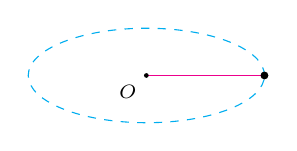
\begin{tikzpicture}[font=\scriptsize]
	\draw[dashed,cyan] (0,0) ellipse(1.5 and .6);
	\draw[magenta] (0,0)--(1.5,0);
	\fill (0,0)node[below left]{\(O\)} circle(.03) (1.5,0) circle(.05);
\end{tikzpicture}
\begin{choices}
	\item 圆周运动轨道可处于任意平面内
	\item 小球的质量为 \( \frac{FR^2}{4\pi^2 n^2} \)
	\item 若误将 \( n-1 \) 圈记作 \( n \) 圈，则所得质量偏大
	\item 若测 \( R \) 时未计入小球半径，则所得质量偏小
\end{choices}
\begin{answer}
	A\qquad 提示：太空实验室完全失重
\end{answer}